\subsection{$\lambda$ parameters}
\label{sec:LambdaParams}

\subsubsection{Thermal yield estimates}
\label{sec:ThermalYields}

THERMINATOR, using efficiencies, yields, fakes






\subsubsection{Reconstruction efficiency effects on relative particle yields}
\label{sec:ReconstructionEff}

In this section we discuss how to use Monte Carlo events with detector effects to estimate reconstruction efficiency.  
The reconstruction efficiency will be an important component in our subsequent estimation of $\lambda$ parameters.

$\Lambda$ arise from many different sources.
There are primary $\Lambda$; $\Lambda$ resulting from $\Sigma$ decays and the decays of short-lived resonances, which cannot be distinguished from primary $\Lambda$; and $Lambda$ coming from the weak decays of $\Xi$ and $\Omega$ baryons, some of which can be removed via topological cuts.
Detector efficiencies and topological reconstruction cuts alter the yields of $\Lambda$ from these various sources in different ways.
To investigate the influence of reconstruction efficiencies on particle yields, we looked at the reconstruction rates of the different particle types using the HIJING run specified in Section \ref{sec:DataSelection}.  
The MC-truth yields of the V0s were examined at three stages of reconstruction:
\begin{enumerate}
\item In the raw MC event before any detector simulation was added to the MC particles.  
Here the daughters of the V0s are required to be in mid-rapidity and surpass a minimum $p_\mathrm{T}$ value, so as to only look at findable V0s.
\item In the V0 finder before any analysis-side reconstruction cuts were employed.
\item After topological reconstruction cuts were made.
\end{enumerate}
At each stage, the MC truths of all remaining particles of the following types were counted: primary $\Lambda$; secondary $\Lambda$ from $\Sigma^0$, $\Sigma^*$, $\Xi^0$, $\Xi^-$, $\Omega$, and other sources; the respective anti-particles; $\mathrm{K}^0_{\mathrm{S}}$ misidentified as $\Lambda$ or $\bar{\Lambda}$; other misidentified V0s; and fake V0s reconstructed in the V0 finder.  
The resulting yields are visible in Figure \ref{fig:MCYields}.

\begin{figure}[hbtp]
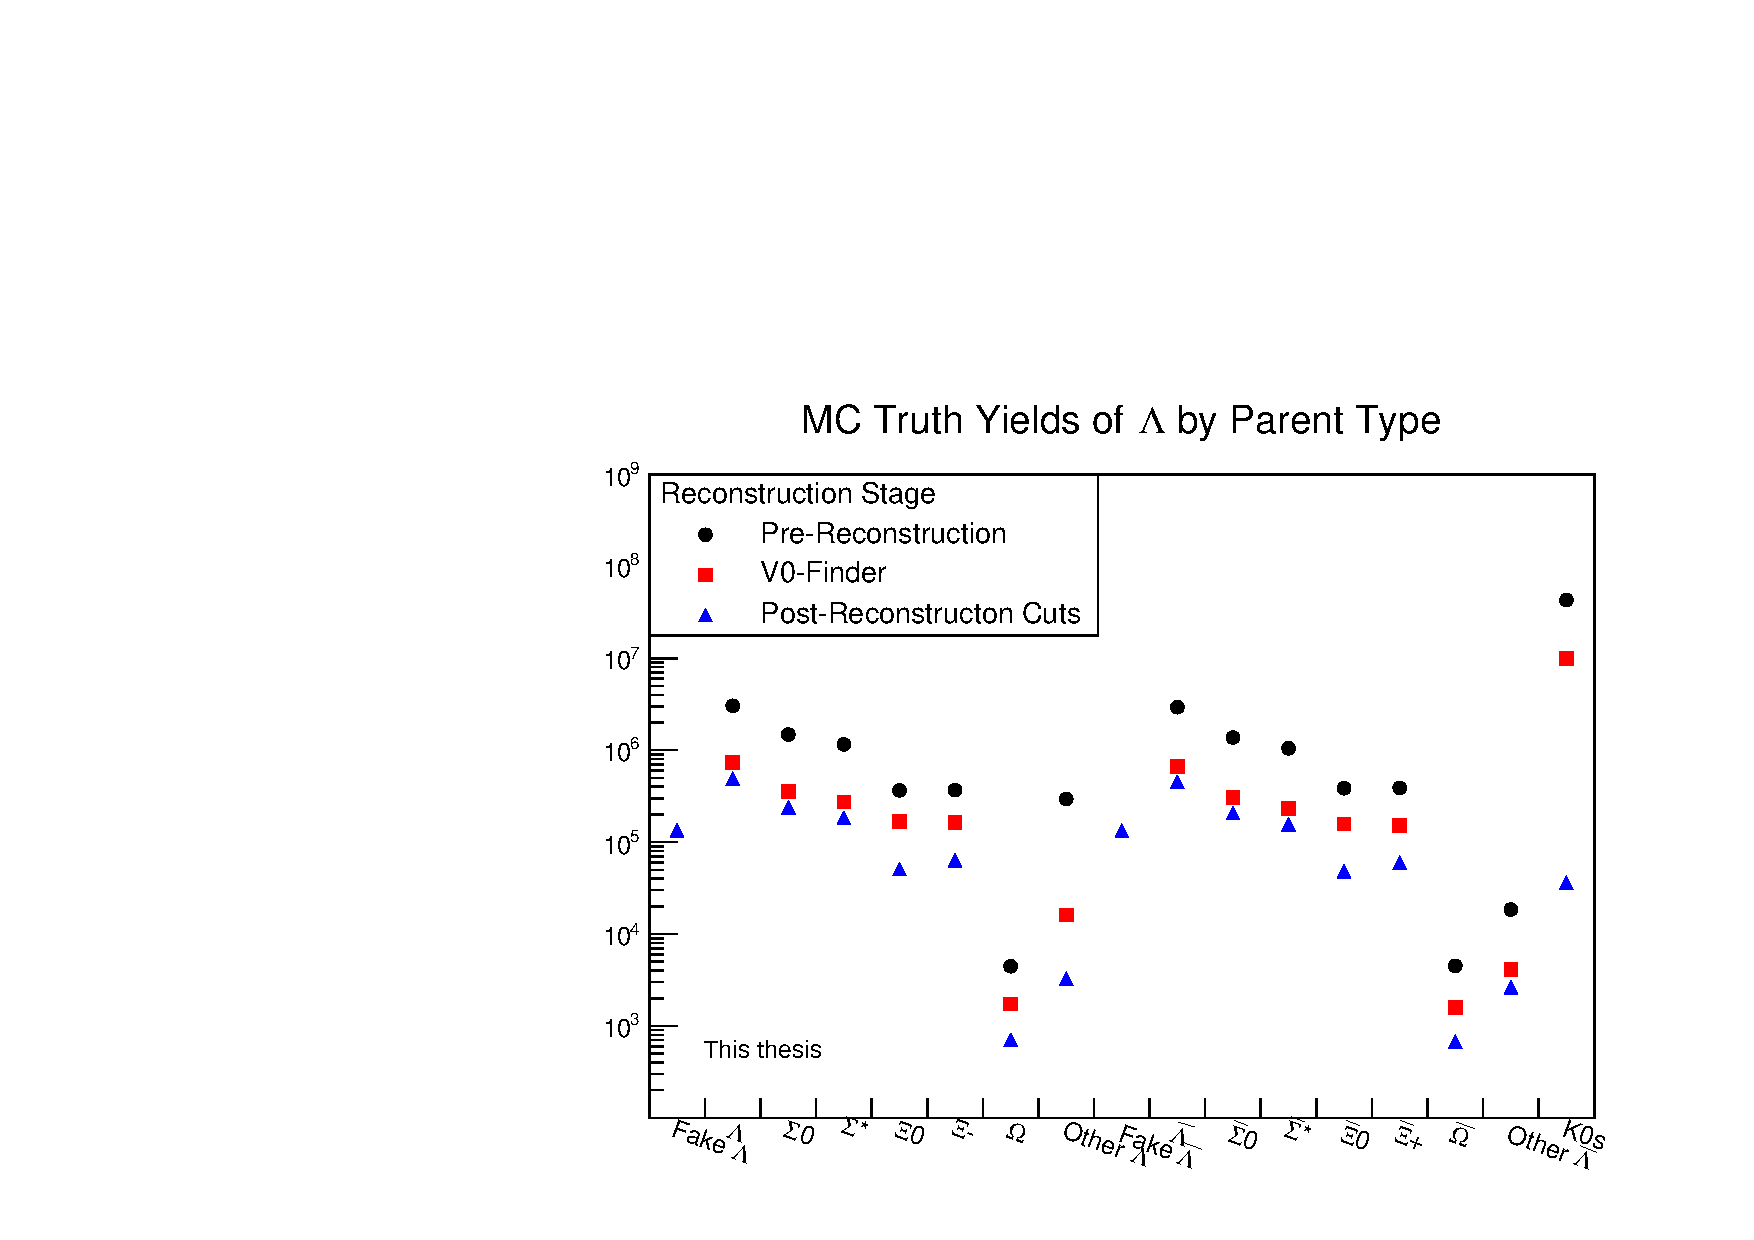
\includegraphics[width=36pc]{Figures/2014-02-03-MCYields.pdf}
\caption[$\Lambda$ MC Yields at Different Reconstruction Stages]{
MC truth yields of $\Lambda$ at different stages of reconstruction.
The x-axis shows the parentage of the reconstructed particle. 
The $\Lambda$ and $\bar{\Lambda}$ bins are primary particle yields.  
Other bins show the number of $\Lambda$ ($\bar{\Lambda}$) that come from decays of other particles. 
The $\mathrm{K^0_s}$ bin shows the number of kaons that were misidentified as $\Lambda$ and $\bar{\Lambda}$.
The black points show the yields that exist in the underlying event, the red points show the true parentage of V0-candidates that have been found by the offline V0 finder, and the blue points show yields after all topological reconstruction cuts have been imposed.
Only midrapidity particles that exceed a minimum $p_\mathrm{T}$ cut have been examined, and injected signals have been excluded from this analysis.}
\label{fig:MCYields}
\end{figure}

The results of Figure \ref{fig:MCYields} can be better interpreted by taking the ratios of the yields at different stages.  
Figure \ref{fig:V0ToMassCut} shows one such ratio.  Here, one can see the fraction of V0s in the V0 finder that survived all the reconstruction cuts.  
From this, one can see how successful the current topological cuts are at selecting (anti)$\Lambda$ of various origins.  
With different topological cuts made, a before-and-after comparison of this plot shows the efficacy of the new cuts at removing secondary V0s vs primary V0s, as in Figure \ref{V0ToMassCutWithDifferentVarBin}.

Figure \ref{fig:OriginToMassCut} shows another ratio.  
In this plot, one sees the event-averaged reconstruction efficiency from the beginning (particles in the underlying event) to the end (all particles passing all cuts).  
This efficiency encompasses not only the results of the analysis-side cuts, but also the natural tracking efficiencies of ALICE detector.  
One can see that the various $\Lambda$ and $\bar{\Lambda}$ types for the most part have a reconstruction rate between 15-25\%.  
These reconstruction efficiencies could be convoluted with the thermal yield calculations of Section \ref{sec:LambdaParams} to obtain corrected estimates of the yields and $\lambda$ parameters.  
Further analyses of these results are in progress.

\subsubsection{A note on injected Monte Carlo signals}
\label{sec:InjectedMCSignals}

It should be noted that this MC run, LHC12a17a\_fix, has injected $\Xi^0$, $\Xi^-$, and $\Omega$ signals, but not their respective antiparticles.  T
he disparity can be seen in Figure \ref{fig:MCEfficiencyWithInjected}, which shows the average reconstruction efficiencies of $\Lambda$ ($\bar{\Lambda}$) broken down in terms of the Monte Carlo truth of each V0's parent species. 
The reconstruction efficiency is defined as the ratio of the number of reconstructed $\Lambda$ ($\bar{\Lambda}$) of each origin type versus the number of V0 candidates of each origin in the V0 finder.  
A clear disparity can be seen between the reconstruction efficiencies of $\Lambda_{\Xi}$ and $\Lambda_{\Omega}$ and their respective antiparticles.  
(This plot is a few months out of date - the reconstruction cuts employed in this figure are somewhat looser than those employed in the current analysis.)

The origin of this disparity has not been investigated in great detail, though it is suspected that the disparity arises from differences between the $p_\mathrm{T}$ spectra of the injected V0s and the underlying HIJING particles.  
Because the efficacy of the various reconstruction cuts and the detector efficiency is $p_\mathrm{T}$ dependant, the average reconstruction efficiency of injected particles may differ from the base HIJING particles.  
Figure \ref{fig:MCEfficiencyWithInjected} therefore shows a disparity between multistrange hyperon and antihyperon efficiency because the hyperons include a mix of injected and underlying particles, while the antihyperons come only from the underlying event. 
The analysis was performed again with injected signals removed (see Figure \ref{fig:MCEfficiencyNoInjected}).  
Without the injected signals, reconstruction efficiencies for the multi-strange particles and anti-particles are seen to be in line.  
Subsequent studies of reconstruction cuts and efficiency were performed without injected signals such that secondary $\Lambda$ and $\bar{\Lambda}$ efficiencies would be consistent.

\begin{figure}[hbtp]
\includegraphics[width=36pc]{Figures/2014-04-20-Efficiency-WithInjectedSignals-OldCuts_2013-09-04Run.pdf}
\caption[$Lambda$ reconstruction efficiencies with injected signals]{Average reconstruction efficiencies of $\Lambda$ ($\bar{\Lambda}$) broken down in terms of the Monte Carlo truth of each V0's parent species.  
Reconstruction efficiency is defined as the ratio of the number of reconstructed $\Lambda$ ($\bar{\Lambda}$) of each origin type versus the number of V0 candidates of each origin in the V0 finder.  
The analysis was performed for HIJING events with injected hyperon signals.  
The events included injected $\Lambda$, $\bar{\Lambda}$, $\Xi$, and $\Omega$, but no $\bar{\Xi}$ or $\bar{\Omega}$.  
A clear disparity can be seen between the reconstruction efficiencies of $\Lambda_{\Xi}$ and $\Lambda_{\Omega}$ and their respective antiparticles.  
This plot is a few months out of date - the reconstruction cuts employed in this figure are somewhat looser than those employed in the current analysis.}
\label{fig:MCEfficiencyWithInjected}
\end{figure}

\begin{figure}[hbtp]
\includegraphics[width=36pc]{Figures/2014-04-20-Efficiency-NoInjectedSignals-OldCuts_2013-11-19Run.pdf}
\caption[$Lambda$ reconstruction efficiencies without injected signals]{Average reconstruction efficiencies of $\Lambda$ ($\bar{\Lambda}$) broken down in terms of the Monte Carlo truth of each V0's parent species.  
Reconstruction efficiency is defined as the ratio of the number of reconstructed $\Lambda$ ($\bar{\Lambda}$) of each origin type versus the number of V0 candidates of each origin in the V0 finder.  
The analysis was performed for HIJING events with injected hyperon signals.  
However, injected hyperon signals have been excluded from this plot.  
The various secondary $\Lambda$ are seen to have approximately the same reconstruction efficiency as respective antiparticles.  
This plot is a few months out of date - the reconstruction cuts employed in this figure are somewhat looser than those employed in the current analysis.}
\label{fig:MCEfficiencyNoInjected}
\end{figure}




\subsubsection{Estimates of \texorpdfstring{$\lambda$}{lambda} parameters}
\label{sec:LambdaParamEstimates}

In this section, we estimate of the relevant $\lambda$ parameters involved in fitting these systems.  
$\lambda$ can roughly be understood to be the pair purity of the system that is being fit, i.e.\ the fraction of true pairs over total pairs.  
There are additional factors that can affect $\lambda$ such as source coherence or non-gaussianity of underlying source, but these complications will be neglected in this analysis.

Many femtoscopic analyses utilize a single $\lambda$ value in their fit procedure as an indication of their overall pair purity.  
This is fine in the cases where the impure pairs (i.e.\ the other $1 - \lambda$ fraction of pairs) are uncorrelated.
But if there are residual correlations, then it becomes necessary estimate their contributions to the correlation function.
Additional $\lambda$ parameters can be attributed to each residual correlation according to the fraction of total pairs of that type.
In principle, all these $\lambda$ can be left as free fit parameters.
In practice, that results in fits that are far too unconstrained to converge properly.
In this analysis, we will estimate the $\lambda$ parameters for each relevant residual correlation, and use those numbers as fixed parameters in the fit.

%A more refined estimate could be made by convoluting ALICE particle spectra with analysis-specific reconstruction efficiencies to determine analysis-specific yields of the various particle types.  
%That avenue will be discussed more in Section \ref{sec:ReconstructionEff}. 

To understand the mathematical motivation behind the $\lambda$ parameters, let us consider the simple case where the signal pairs of the correlation function come from a single event.  
Within this event, all combinations of reconstructed V0s are paired together and binned according to their $k^*$ values.  
For this simple example, let's assume that the reconstructed V0s consist of primary $\Lambda$, secondary $\Lambda$, and fake $\Lambda$.  
Let us assume that origin of the different $\Lambda$ cannot be determined - the analysis only knows that a given V0 appears to be a $\Lambda$.  
As mentioned above, the total correlation function will be a linear combination of the component correlation functions (primary-primary, primary-secondary, primary-fake, fake-fake, etc.).  
The $\lambda$ parameters for each component correlation are given by the fraction of total pairs of that type.  
For example, if there are ten distinct $\Lambda\Sigma$ pairs and one hundred total pairs, then $\lambda_{\Lambda\Sigma} = 1/10$.  
If all pair types are accounted for, 
\begin{equation}
\label{eq:SumLambdaUnity}
\sum\limits_{ij}\lambda_{ij} = 1.
\end{equation}

We can use the following equations to estimate the $\lambda$ parameters for different types of pairs. 
These equations take the general form 
\begin{equation}
\lambda = \frac{\mathrm{Specific Pairs}}{\mathrm{Total Pairs}},
\end{equation}
where the calculations for numbers of pairs are simple combinatorics.  If more than one event is being used (as is the case in the data), the equation becomes
\begin{equation}
\lambda = \frac{\langle\mathrm{Specific Pairs}\rangle}{\langle\mathrm{Total Pairs}\rangle},
\end{equation}
where the average is done over events.

The $\lambda$ parameter for two identical particles (e.g. both primary $\Lambda$) is given by
\begin{equation}
\label{eq:LambdaIdentical}
\lambda_{ii} = \frac{N_i}{T}\frac{(N_i -1)/2}{(T-1)/2} = \frac{N_i}{T}\frac{(N_i -1)}{(T-1)}
\end{equation}
where $N_i$ is the number of particles of species $i$, $T = \sum\limits_i N_i$ is the total number of particles, and the factors of $1/2$ remove double counting.  
For two particles with different origins (e.g. a primary $\Lambda$ and a $\Lambda$ from a $\Sigma^0$ decay)
\begin{equation}
\lambda_{ij} = \frac{N_i}{T} \frac{N_j}{(T-1)/2}
\end{equation}
for $i \neq j$.  
$\lambda$ can also be calculated for pairs that are distinguishable, such as primary $\Lambda$ and primary $\bar{\Lambda}$:
\begin{equation}
\lambda_{i\bar{j}} = \frac{N_i N_{\bar{j}}}{T\bar{T}}
\end{equation}
where $T$ is the sum of all indistinguishable particles and $\bar{T}$ is the sum of all indistinguishable antiparticles.



%One should note here that the above $\lambda$ equations technically apply to some sort of single-event correlation function.  
%The $\lambda$ parameters measured or estimated for a million-event correlation function would roughly correspond to an event-averaged value.  
%Nonetheless, we can attempt to employ these formulae to obtain ballpark estimates of the $\lambda$ parameters, given estimates of the yields of each type of particle.
%
%As the goal of this analysis is to measure the correlations of primary $\Lambda$, it is important to know the relative yields of secondary $\Lambda$.  
%We can obtain an estimate \cite{Florkowski:2010zz} of the yields of different types of particles at mid-rapidity from a thermal model using
%\begin{equation}
%\frac{1}{m_{\mathrm{T}}}\frac{dN}{dm_{\mathrm{T}}} \propto \exp{(-m_\mathrm{T}/T)}
%\end{equation}
%where the transverse mass $m_\mathrm{T} = \sqrt{m^2_{\mathrm{inv}} + p^2_{\mathrm{T}}}$ and $T$ is the chemical-feezeout temperature.  
%Integrating over $m_\mathrm{T}$ gives $N \propto (m_\mathrm{inv} + T) \exp{(-m_\mathrm{inv}/T)}$.  
%Therefore, the yield of any particle species $i$ relative to the $\Lambda$ yield is
%\begin{equation}
%\frac{N_i}{N_\Lambda} \approx \frac{m_i + T}{m_\Lambda + T} \exp{((m_\Lambda - m_i)/T)}.
%\end{equation}
%
%Particles that decay into $\Lambda$ include $\Sigma^0$, $\Xi^0$, $\Xi^-$, and $\Omega^-$.  
%Assuming a freezeout temperature of 165 MeV, and taking into account that the $\Omega$ has a branching ratio of ~68\% and the others ~100\%, we can then estimate that for every 100 $\Lambda$, there will be approximately 67 $\Sigma$, 34 of each type of $\Xi$, and 3 $\Omega$.
%
%Before calculating the $\lambda$ parameters, it is also necessary to know approximately how many fake $\Lambda$ there are.  
%In Section \ref{sec:Recon}, we estimated that our signal quality $P$ was $P = real/(real + background) \approx 0.82$ (Note: calculations were performed using a now outdated purity estimate).  
%Taking $real$ to be the sum of all the primary and secondary $\Lambda$, we calculate that $\frac{background}{real} = P^{-1}-1 \approx 0.22$.  
%With the above yields totalling 238 $\Lambda$, we would expect to see an additional 52 fake $\Lambda$.  
%Based on these values, we can now estimate the $\lambda$ parameters for all pair types.
%
%\begin{center}
%\begin{tabular}{|l|l|c|}
%\hline
%					& 	$\lambda$	&	Cumulative total \\ \hline
%$\Lambda\Lambda$   	&	0.12			&	0.12 \\ \hline
%$\Lambda\Sigma^0$  	&	0.16			&	0.28 \\ \hline
%$\Lambda\Xi^0$     	&	0.08			&	0.36 \\ \hline
%$\Lambda\Xi^-$     	&	0.08			&	0.44 \\ \hline
%$\Lambda\Omega$    	&	0.007		&	0.45 \\ \hline
%$\Sigma^0\Sigma^0$ 	&	0.05			&	0.50 \\ \hline
%$\Sigma^0\Xi^0$    	&	0.05			&	0.55 \\ \hline
%$\Sigma^0\Xi^-$    	&	0.05			&	0.61 \\ \hline
%$\Sigma^0\Omega$   	&	0.004		&	0.61 \\ \hline
%$\Xi^0\Xi^0$       	&	0.01			&	0.63 \\ \hline
%$\Xi^0\Xi^-$ 		&	0.03			&	0.65 \\ \hline
%$\Xi^0\Omega$ 		&	0.002		&	0.66 \\ \hline
%$\Xi^-\Xi^-$ 		&	0.01			&	0.67 \\ \hline
%$\Xi^-\Omega$ 		&	0.002		&	0.67 \\ \hline
%$\Omega\Omega$ 		&	0.00			&	0.67 \\ \hline
%\end{tabular}
%\end{center}
%
%These estimates have several interesting characteristics.  
%First, the sum of the primary correlation all the residual correlations totals to 0.67.  
%The other 33\% is lost to the background.  
%Note that feedup from residual p$\Lambda$ correlations would be included in this 33\%, though feedup has otherwise not yet been explored in this analysis. 
%Another striking feature of these data is that the contribution from $\Lambda\Sigma$ is actually larger than the contribution from $\Lambda\Lambda$.  
%In other words, if the hyperon yields and reconstruction efficiencies of the true PbPb data are reminiscent of the yields above, then this analysis is measuring the $\Lambda\Sigma$ correlation more than the $\Lambda\Lambda$ correlation.  
%It should also be noted that contributions from $\Lambda\Xi$, $\Sigma\Sigma$, and $\Sigma\Xi$ are appreciable.
%
%For the the $\Lambda\bar{\Lambda}$ analysis, estimates of the $\lambda$ parameters work out to be approximately the same as in the table above.
